\documentclass{beamer}

\usepackage{mpemath}
\usepackage{subcaption}
\usepackage[normalem]{ulem}
\usepackage{amsmath}
\usepackage{amssymb}
\usepackage{mathtools}
\usepackage{pgf}
\usepackage{pgfplots}
\usepackage{tikz}
\usepackage{booktabs}
\usepackage{siunitx}
\usepackage{natbib}
\usepackage{tabularx}
\usepackage{multirow}
\usepackage{amsmath}
\usepackage{mathtools}
\usepackage{amssymb}
\usepackage{bbm}


\usetikzlibrary{arrows,automata,backgrounds,positioning,decorations,intersections,matrix}

% *** Styles ***
\usetheme{Singapore}
\setbeamertemplate{navigation symbols}{}
% \usetheme[progressbar=frametitle]{metropolis}
% \usecolortheme{dolphin}
%\useinnertheme{circles}
%\usecolortheme{rose}
%\setbeamercovered{transparent}
\setbeamercovered{invisible}
\usefonttheme{professionalfonts}
%\usefonttheme[onlymath]{serif}
\setbeamertemplate{footline}[frame number]

\title{ROIL -- Robust Offline Imitation Learning}
\author{Gersi Doko}
\institute{Department of Computer Science \\ University of New Hampshire}
% \date{2024}

\AtBeginSection[]{
	\begin{frame}
          \vfill
	\centering
	% \usebeamerfont{title}
        {\huge\bf \insertsectionhead}%
	\vfill
\end{frame}
}

\begin{document}

\frame{\titlepage}

\section*{Intro}

\begin{frame}
	\frametitle{Robust Offline Imitation Learning}
	\textbf{Objective}: Learn a policy from expert demonstrations
	\begin{itemize}
	\item Health care: automating and improving ER care
	\item Robotics: self-driving cars, complete tasks only from demonstrations
	\item Retail: recommendation systems, customer service
	
	\end{itemize}
	\vfill
	\textbf{Offline IL}: Compute policy from a fixed dataset of expert demonstrations
	\begin{itemize}
		\item No interaction with the environment
	\end{itemize}
\end{frame}

\begin{frame}
	\frametitle{This Talk}
	Computing policies that minimize worst case regret, with respect to the worst case expert

	\vfill
	\emph{Key Idea}: Generate a convex set of consistent experts, then minimize regret

	\textbf{Outline}
	\begin{itemize}
	\item \emph{Motivation}: Why study IRL?
	\item \emph{Domain Introduction}: What is IRL?
	\item \emph{Robust Offline IL}: New approach to solving the robust IRL objective
	\end{itemize}
\end{frame}

\section*{Motivation}

\begin{frame}
\frametitle{Motivation}
	\begin{itemize}
		\item Solve problems where it's hard to define what outcome we want
		\item Self-driving, Robotic Control, Medicine, Recommendation Systems, etc.
		\item Often have access to expert demonstrations instead of a clear description for the task
	\end{itemize}
\end{frame}

\begin{frame}
\frametitle{Motivation}
	\begin{itemize}
		\item Similar to Reinforcement Learning, but we don't have access to the true reward function $r^\star : \mathcal{S} \times \mathcal{A} \to \Real$
		\item Instead, we try and replicate the experts' behavior given their demonstrations $D_e = (s_i, \pi_e(s_i))_{i=1}^N$
		\item Generally demonstrations are given as state-action pairs collected along expert trajectories with horizon $N$
		\item We make no assumptions on the experts' optimality, nor the temporal structure of the demonstrations
	\end{itemize}
\end{frame}

\begin{frame}
\frametitle{Motivation}
Two approaches to learning from demonstrations:
\begin{itemize}
	\item \emph{Inverse Reinforcement Learning (IRL)}: Learn a reward function from expert demonstrations then use RL to learn a policy
	\item \emph{Imitation Learning (IL)}: Learn a policy directly from expert demonstrations
\end{itemize}
\textbf{Distinction}: Inverse Reinforcement Learning (IRL) \emph{typically} assumes problem dynamics are known, Imitation Learning (IL) \emph{typically} does not
\end{frame}

\section*{Domain Introduction}

\begin{frame}
	\frametitle{Notation}
	\begin{itemize}
		\item Let m, n be positive integers
		\item $\Real^{mn}$ denotes the set of $m \cdot n$-dimensional real vectors
		\item $\Real^{m \times n}$ denotes the set of $m \times n$ real matrices
		\item $\Delta^m$ denotes the $m$-dimensional probability simplex
		\item $\Pi$ denotes the set of all randomized markov policies
	\end{itemize}
\end{frame}

\begin{frame}
\frametitle{Domain Introduction}
	\begin{itemize}
		\item Our work falls into the Inverse Reinforcement Learning (IRL) category since we assume access to model dynamics
		\item We do not attempt to learn the expert's reward function
		\item Instead, we aim to learn a policy that minimizes the regret with respect to the \emph{worst case expert} consistent with the demonstrations $D_e$
	\end{itemize}
\end{frame}

\begin{frame} \frametitle{Markov Decision Process}
  \textbf{Model} (tabular in this talk) \par
    {\small
   ~~~States $\mathcal{S}$: $s_1, s_2, s_3, \dots $ \par
   ~~~Actions $\mathcal{A}$: $a_1, a_2, \dots $ \par
   ~~~Transition probabilities $\mathcal{P} \in \Real^{\mathcal{S} \times \mathcal{A} \times \mathcal{S} }$ \par
   ~~~Initial state distribution $p_0 \in \Delta^\mathcal{S}$ \par
   ~~~Discount factor $\gamma \in \Real$ \par
   ~~~\sout{Rewards $r \in \Real^{\mathcal{S} \times \mathcal{A}}$}}
    \vfill 
    \textbf{Solution}: Policy ${\pi}\colon \mathcal{S} \to \Delta^\mathcal{A}$
    \vfill
    \textbf{Return}: Discounted expected infinite horizon return (expectation over trajectories):
    \[
	    \tilde{\rho}(\pi) = \lim_{T \to \infty} \sum_{t=0}^T \gamma^t r(\tilde{s}^{\pi}_t, \tilde{a}^{{\pi}}_t)
    \]
    \vfill
    \textbf{Random variables}: $\tilde{\rho}, \tilde{s}, \tilde{a}, \tilde{x}, \dots $ adorned with tilde
\end{frame}

\begin{frame}
	\frametitle{Domain Introduction}
	\begin{itemize}
		\item In addition to the MDP, we are given a matrix of features $\Phi \in \Real^{\mathcal{S}\mathcal{A} \times k}$
		\item Features are typically constructed by human experts and enable generalization across unseen states
		\item We are also given a dataset of state, action pairs $D_e$ generated by some expert policy $\pi_e$. \[ D_e = (s_i, \pi_e(s_i))_{i=1}^N \]
		\item Notice we make no assumptions on the state visitation frequency of the expert,
			the expert may choose to show us only a subset of the state space
	\end{itemize}
\end{frame}

\begin{frame}
	\frametitle{Domain Introduction}
\begin{itemize}
	\item $\pi_e$ follows some unknown reward function $r^\star : \mathcal{S} \times \mathcal{A} \to \Real$.
\end{itemize}
	\emph{Common assumption} : $r^\star$ can be realized by our features $\Phi \in \Real^{\mathcal{S}\mathcal{A}} \times k$
	and a weight vector $w \in \mathcal{W}$ such that $r^\star = \Phi w$.

	Prior work has restricted the weight vector to the L1 norm ball:
	\[ \mathcal{W} = \lbrace w \in \Real^k \mid \lvert \lvert w \rvert \rvert_1 \leq 1 \rbrace \]
	There are other viable choices of $\mathcal{W}$, which we accommodate for as an extension to our work.
\end{frame}


\section*{Our Approach}

\begin{frame}
	\frametitle{Our Approach}
	\textbf{Problem}: Find a policy $\pi$ that minimizes the regret with respect to the worst case expert consistent with the demonstrations $D_e$.
	\[ \rho(\tilde{\pi}, r) = \lim_{t \to \infty} \mathbb{E}^{\tilde{\pi}, \mathcal{P}} \lbrack \sum_{t=0}^T \gamma^t r(\tilde{s_t}, \tilde{\pi}(\tilde{s_t})) \rbrack \]
\end{frame}

\begin{frame}
	\frametitle{Our Approach}
	\textbf{Problem}: Find a policy $\pi$ that minimizes the regret with respect to the worst case expert consistent with the demonstrations $D_e$.
	\[ \rho(\tilde{\pi}, r) = \lim_{t \to \infty} \mathbb{E}^{\tilde{\pi}, \mathcal{P}} \lbrack \sum_{t=0}^T \gamma^t r(\tilde{s_t}, \tilde{\pi}(\tilde{s_t})) \rbrack \]
	\[ \Pi_R(D) = \lbrace \pi \in \Pi \mid \pi(s,a) = 1 \quad \forall (s,a) \in D \rbrace \]
\end{frame}


\begin{frame}
	\frametitle{Our Approach}
	\textbf{Problem}: Find a policy $\pi$ that minimizes the regret with respect to the worst case expert consistent with the demonstrations $D_e$.
	\[ \rho(\tilde{\pi}, r) = \lim_{t \to \infty} \mathbb{E}^{\tilde{\pi}, \mathcal{P}} \lbrack \gamma^t r(\tilde{s_t}, \tilde{\pi}(\tilde{s_t})) \rbrack \]
	\[ \Pi_R(D) = \lbrace \pi \in \Pi \mid \pi(s,a) = 1 \quad \forall (s,a) \in D \rbrace \]
	\[ \min_{\pi \in \Pi_R(D_e)} \max_{\pi_e \in \Pi_R(D_e)} \max_{r \in \mathcal{R}} \rho(\pi_e, r) - \rho(\pi, r)\]
\end{frame}

\begin{frame}
	\frametitle{Our Approach}
	\[ \min_{\pi \in \Pi} \max_{\pi_e \in \Pi_R(D_e)} \max_{r \in \mathcal{R}} \rho(\pi_e, r) - \rho(\pi, r)\]
	\textbf{Observation}: The maximization over $\mathcal{R}$ may result in an intractable optimization problem.
	\textbf{Solution}: Recall the set of possible reward functions.
        \[ \mathcal{W} = \lbrace w \in \Real^k \mid \lvert \lvert w \rvert \rvert_1 \leq 1 \rbrace \]
	\[ \mathcal{R} = \lbrace r \in \Real^{\mathcal{S} \mathcal{A}} \mid \exists w \in \mathcal{W}, \; r = \Phi w \rbrace \]
	\[ \min_{\pi \in \Pi_R(D_e)} \max_{\pi_e \in \Pi_R(D_e)} \max_{w \in \mathcal{W}} \rho(\pi_e, \Phi w) - \rho(\pi, \Phi w)\]
\end{frame}

\begin{frame}
	\frametitle{Our Approach}
	\textbf{Implementation Detail}: It can be difficult in practice to optimize over $\Pi$, and $\Pi_R(D_e)$ directly.\\
	\textbf{Solution}: Instead optimize over the occupancy frequencies of the policies.
	\[ \mathcal{U} = \lbrace u \in \RealPlus^{\mathcal{SA}} \mid \sum_{a \in \mathcal{A}} (I - \gamma \mathcal{P}_a\tr) \cdot u(\cdot, a) = p_0 \rbrace \]
	\[ \Upsilon = \lbrace u \in \mathcal{U} \mid u\tr c = 0 \rbrace \]
	\[ \text{where} \quad c(s,a) =
	\begin{cases}
	1 &\text{if  }
		(s,a) \notin \mathcal{D} \wedge
		\exists a'\in \mathcal{A}, (s, a') \in \mathcal{D}, \\
	0 & \text{otherwise}.
	\end{cases} \]
	\[ \min_{u \in \Upsilon} \max_{u_e \in \Upsilon} \max_{w \in \mathcal{W}} u_e\tr \Phi w - u\tr \Phi w\]
\end{frame}

\section*{ROIL}
\begin{frame}
	\frametitle{ROIL}
	\textbf{ROIL}: Robust Offline Imitation Learning
\[ \begin{mprog}
	\minimize{t \in \Real, u \in \Real^{\mathcal{S} \times \mathcal{A}}} t
	\stc t \geq -u\tr \Phi w + \max_{v \in \Upsilon} v\tr \Phi w,\quad \forall \; w \in ext(\mathcal{W}),
        \cs u\in \Upsilon,
\end{mprog} \]
\vfill

\begin{itemize}
	\item $ext(\mathcal{W})$ is the set of extreme points of $\mathcal{W}$
	\item $u$ is the occupancy frequency of our policy
	\item $t$ is the worst case regret
\end{itemize}
\end{frame}

\begin{frame}
	\frametitle{ROIL-P}
	\begin{itemize}
		\item \textbf{Key Strength}: ROIL does not estimate the occupancy frequency of the expert $\hat{u}_e$
		\item \textbf{Problem}: In On-policy domains, the expert's occupancy frequency is free of covariate shift
		\item \textbf{Solution}: ROIL-P, a variant of ROIL that estimates the expert's occupancy frequency, and prunes the set of reward functions
	\end{itemize}
\end{frame}

\begin{frame}
	\frametitle{ROIL-P}
	\textbf{Solution}: ROIL-P, a variant of ROIL that estimates the expert's occupancy frequency, and prunes the set of reward functions
\[ \begin{mprog}
	\minimize{t \in \Real, u \in \Real^{\mathcal{S} \times \mathcal{A}}} t
	\stc t \geq -u\tr \Phi w + \max_{v \in \Upsilon} v\tr \Phi w,\quad \forall \; w \in ext(\Psi(\mathcal{W})),
        \cs u\in \Upsilon,
\end{mprog} \]

\begin{itemize}
	\item $\Psi(\mathcal{W}) = \lbrace w \in \mathcal{W} \mid \hat{u}_e\tr \Phi w >= 0 \rbrace $
\end{itemize}

\end{frame}

\section*{Experiments}

\begin{frame}
	\frametitle{On-Policy vs Off-Policy}
	\begin{equation*} \label{eq:definition_u_hat}
	\hat{u}_e(s,a)
	\;=\; \sum_{(t, s',a') \in D_e} \gamma^t \cdot  \I{s=s' \wedge\; a=a'},
	\end{equation*}
	\vfill
	\begin{itemize}
		\item \textbf{Definition}: A set of demonstrations $D_e$ is said to be \emph{On Policy} if $$\lim_{N \to \infty} \| \hat{u}_e(D_e^N) - u_e \|_\infty  = 0$$
	\end{itemize}
\end{frame}

\begin{frame}
\frametitle{40x40 Gridworld}

\begin{figure}
  \begin{center}
  \begin{minipage}{0.45\linewidth}
    \centering
    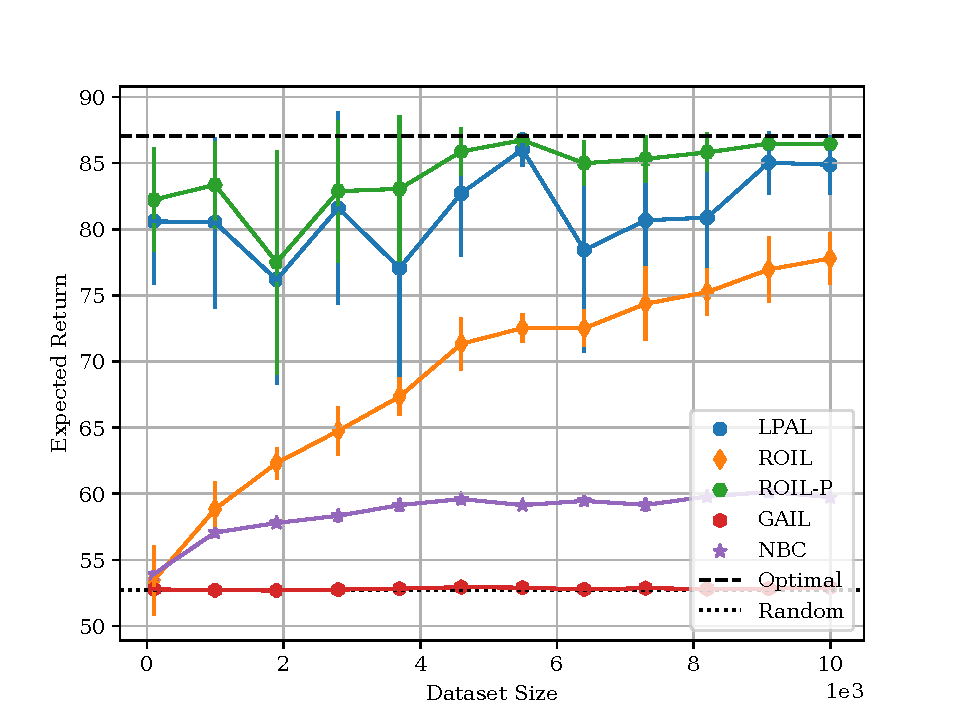
\includegraphics[width=\linewidth]{plots/returns/40x40_gridworld_on_policy_returns.pdf}
    \subcaption{On-Policy}
  \end{minipage}
  \hspace{0.05\linewidth}
  \begin{minipage}{0.45\linewidth}
    \centering
    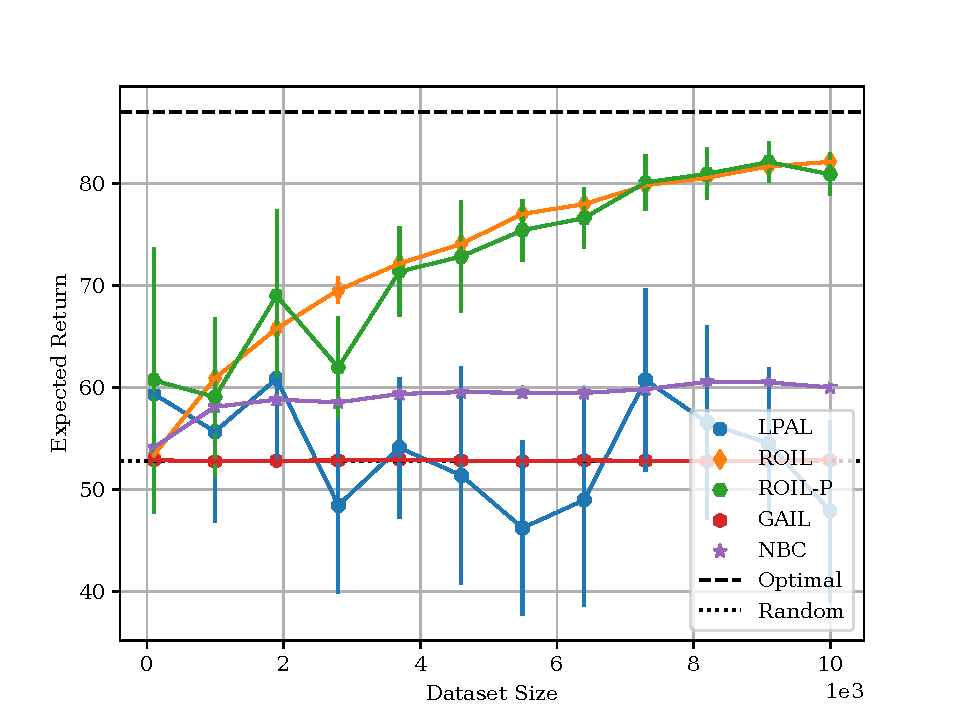
\includegraphics[width=\linewidth]{plots/returns/40x40_gridworld_off_policy_returns.pdf}
    \subcaption{Off-Policy}
  \end{minipage}
  \end{center}
\caption{Returns of All Methods on 40x40 Gridworld}
\end{figure}

\end{frame}

\begin{frame}
	\frametitle{40x40 Driving Simulator}
\begin{figure}
  \begin{center}
  \begin{minipage}{0.45\linewidth}
    \centering
    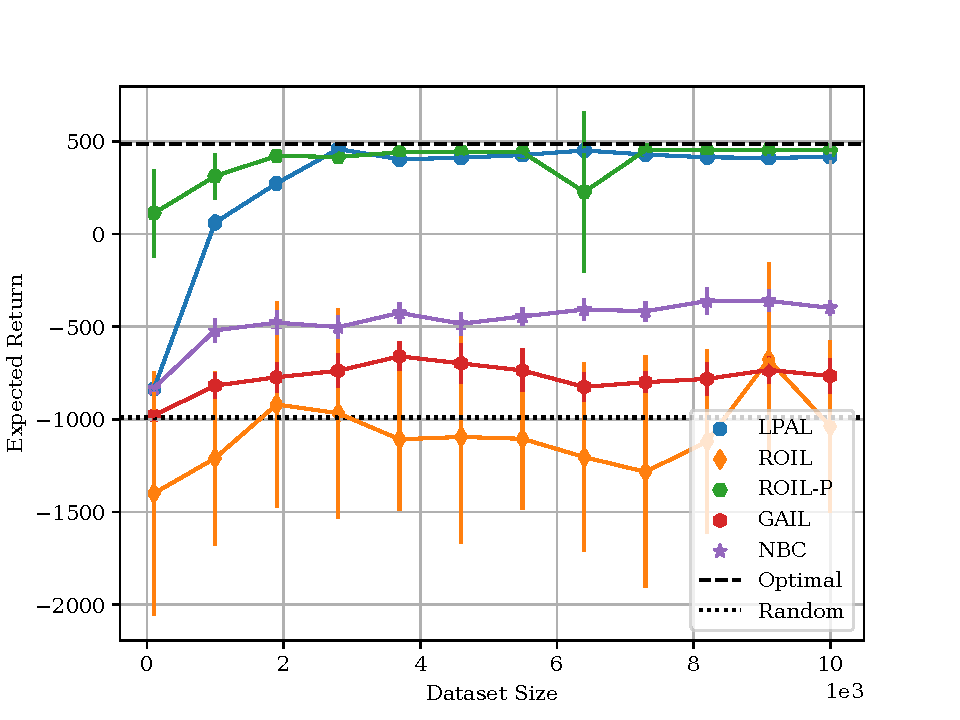
\includegraphics[width=\linewidth]{plots/returns/40x40_driving_on_policy_returns.pdf}
    \subcaption{On-Policy}
  \end{minipage}
  \hspace{0.05\linewidth}
  \begin{minipage}{0.45\linewidth}
    \centering
    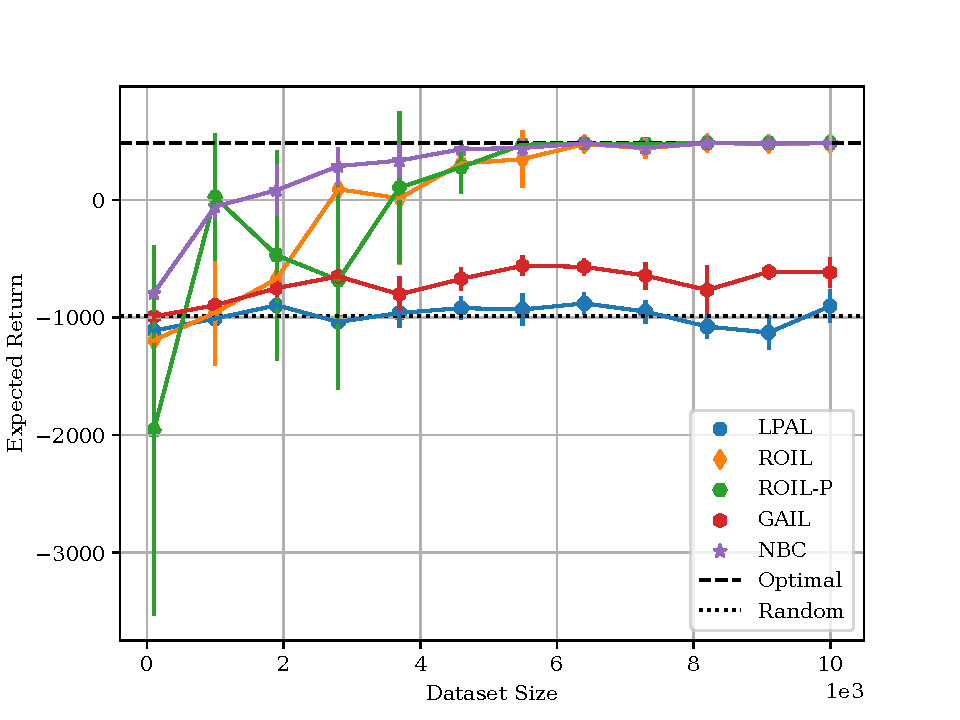
\includegraphics[width=\linewidth]{plots/returns/40x40_driving_off_policy_returns.pdf}
    \subcaption{Off-Policy}
  \end{minipage}
  \end{center}
\caption{Returns of All Methods on 40x40 Driving Simulator}
\end{figure}
\end{frame}

\begin{frame}
\frametitle{Regret Comparison}

 \[ Regret(\pi) = \max_{\pi_e \in \Pi_R(D_e)} \max_{w \in \mathcal{W}} \rho(\pi_e, \Phi w) - \rho(\pi, \Phi w)\]

\begin{figure}
  \begin{center}
  \begin{minipage}{0.45\linewidth}
    \centering
    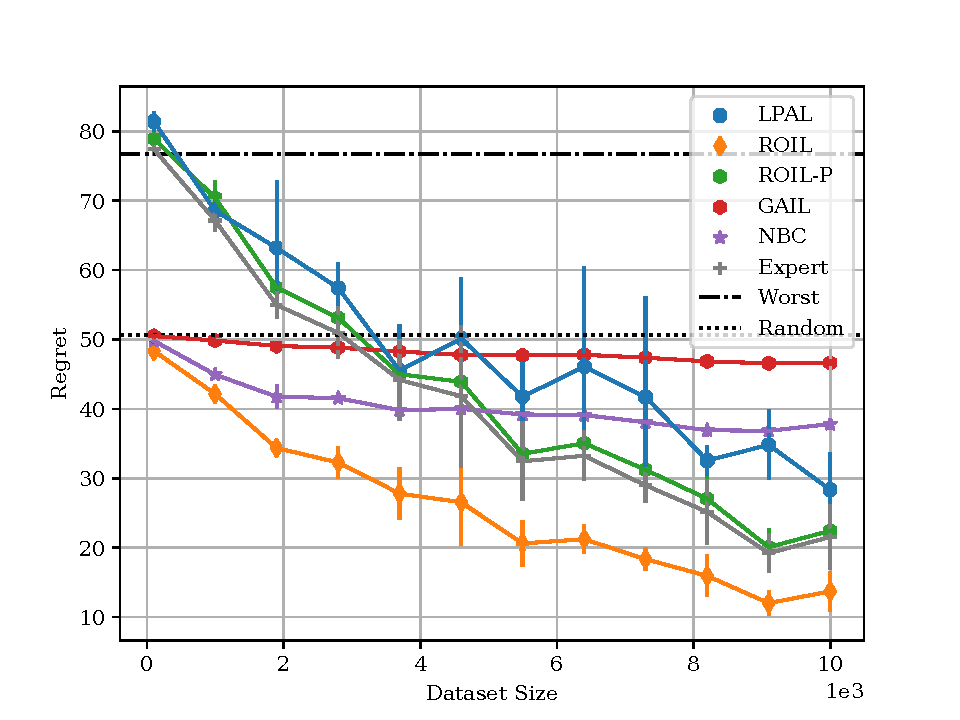
\includegraphics[width=\linewidth]{plots/regrets/40x40_gridworld_on_policy_regret_regrets.pdf}
    \subcaption{On-Policy}
  \end{minipage}
  \hspace{0.05\linewidth}
  \begin{minipage}{0.45\linewidth}
    \centering
    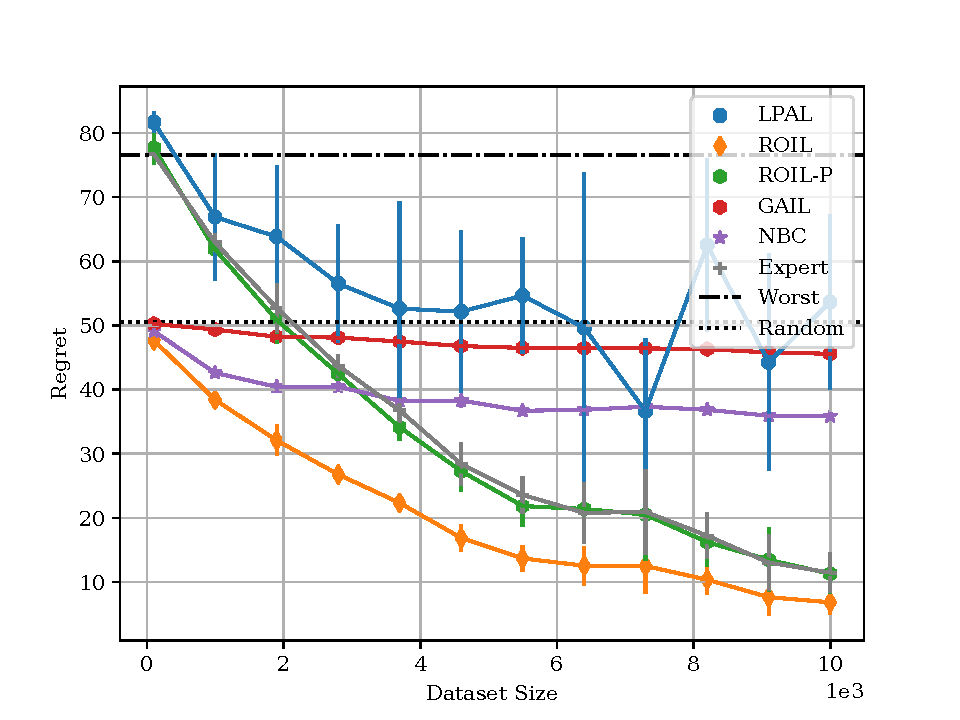
\includegraphics[width=\linewidth]{plots/regrets/40x40_gridworld_off_policy_regret_regrets.pdf}
    \subcaption{Off-Policy}
  \end{minipage}
  \end{center}
\caption{Regret of All Methods on 40x40 Gridworld}
\end{figure}

\end{frame}

\end{document} 
